\documentclass[12pt,letterpaper]{article}

%\pagenumbering{gobble} % arabic, roman, Roman, alph, Alph
\pagenumbering{arabic} % arabic, roman, Roman, alph, Alph
%\setcounter{page}{0} % sets the initial page

\oddsidemargin = -0.25 in
\evensidemargin = -0.25 in
\topmargin = -0.5 in
\headheight = 0 in
%\headsep = 0.5 in
%\topskip = 0 in
\textheight = 9 in
\textwidth = 6.75 in
\footskip = 0.5 in

\usepackage{notes}
\usepackage{graphicx}
\usepackage{tcolorbox}

%\voffset = -0.5 in
%\hoffset = -0.5 in

\parskip 10 pt

\font\sf = cmss10

\setlength\parindent{0pt}




\begin{document}

\thispagestyle{empty}

\baselineskip = 15 pt % between lines

% sanscrif \tt

MATH 180 NOTES \hfill Section 5.4: Indefinite Integrals and the Net Change Theorem

\hrulefill

If $f(x) = x^2 + 2x + 4$, then its derivative is $f'(x) = 2x + 2$. Recall that the function $x^2 + 2x + 4$ is `an' antiderivative of the function $2x + 2$. As the derivative of the constant term is zero, functions $x^2 + 2x + C$, where $C$ can be any constant, would be antiderivatives of the function $2x + 2$. The graphs of functions $x^2 + 2x + C$ are the graph of the function $x^2 + 2x$ shifted vertically by $C$. As there are infinitely many constants $C$, there are infinitely many antiderivatives of the function $2x + 2$.
\begin{center}
\begin{tabular}{lcl}
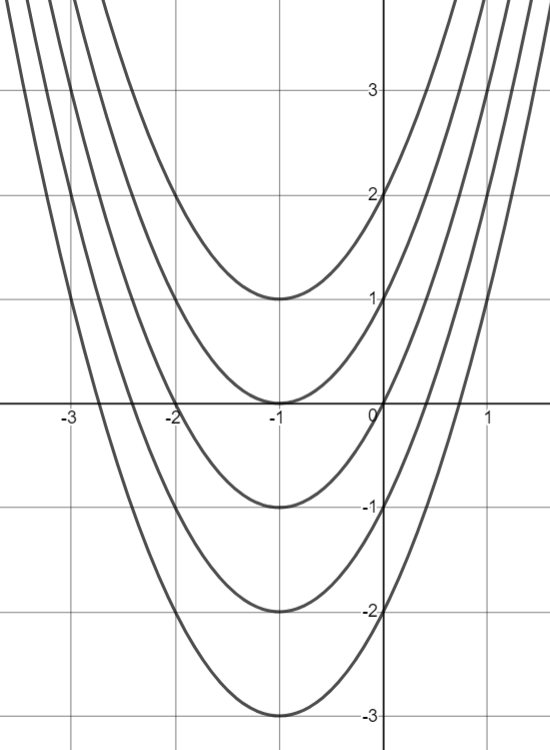
\includegraphics[scale=0.5]{math180_sec5_4_img1.png} & \hspace{30pt} & 
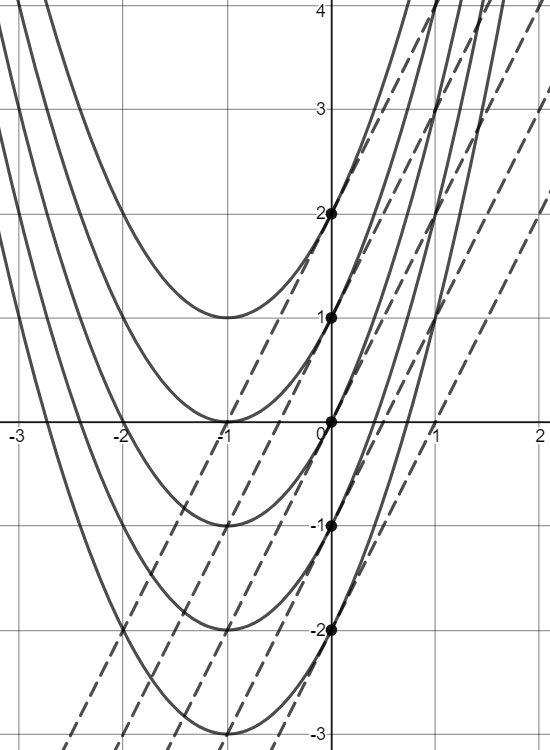
\includegraphics[scale=0.5]{math180_sec5_4_img2.png} \\
Graphs of $y = x^2 + 2x + C$ & & Note that tangents lines at $x = 0$ \\
for $C$ = $-2$, $-1$, $0$, $1$, and $2$ & & are all parallel to each other.
\end{tabular}
\end{center}


\subsection*{Indefinite Integrals}




\begin{tcolorbox}

The set of all antiderivatives of a function $f(x)$ is called the \textbf{indefinite integral} of $f(x)$ and is denoted by $\int f(x) \, dx$.

\end{tcolorbox}

For instance, $\int (2x + 2) \, dx$ is the set of functions $x^2 + 2x + C$ where $C$ is a constant. In a Calculus class, you do not need to specify that ``$C$ is a constant'' as it is understood.
It is very important to note that writing $\int (2x + 2) \, dx = x^2 + 2x$ would be incorrect as the function $x^2 + 2x$ does not represent the all possible set of antiderivatives. So $+ C$ is not optional.

Since $\frac{d}{dx}(\tan(x)) = \sec^2(x)$, the definite integral of $\sec^2(x)$ is $\int \sec^2(x) \, dx = \tan(x) + C$.

Since $\frac{d}{dx}(\log_3(x)) = \frac{1}{\ln(3)x}$, the definite integral of $\frac{1}{\ln(3)x}$ is $\int \frac{1}{\ln(3)x} \, dx = \log_3(x) + C$.

\pagebreak

MATH 180 NOTES \hfill Section 5.4: Indefinite Integrals and the Net Change Theorem

\hrulefill

\begin{center}
Table of Indefinite Integrals

\begin{tabular}{|clclc|}
\hline
&&&&\\
\hspace{5pt} & $\int cf(x) \, dx = c\int f(x) \, dx$ & \hspace{5pt} & $\int (f(x) + g(x)) \, dx = \int f(x) \, dx + \int g(x) \, dx$ & \hspace{5pt} \\
&&&&\\
\hspace{5pt} & $\int k \, dx = kx + C$ & \hspace{5pt} & & \hspace{5pt} \\
&&&&\\
\hspace{5pt} & $\int x^n \, dx = \frac{x^{n+1}}{n+1} + C$ ($n \neq -1$) &  \hspace{5pt} & $\int \frac{1}{x} \, dx = \ln|x| + C$ & \hspace{5pt} \\
&&&&\\
\hspace{5pt} & $\int e^x \, dx = e^x + C$ &  \hspace{5pt} & $\int b^x = \frac{b^x}{\ln(b)} + C$ & \hspace{5pt} \\
&&&&\\
\hspace{5pt} & $\int \sin(x) \, dx = -\cos(x) + C$ &  \hspace{5pt} & $\int \cos(x) \, dx = \sin(x) + C$ & \hspace{5pt} \\
&&&&\\
\hspace{5pt} & $\int \sec^2(x) \, dx = \tan(x) + C$ &  \hspace{5pt} & $\int \csc^2(x) \, dx = -\cot(x) + C$ & \hspace{5pt} \\
&&&&\\
\hspace{5pt} & $\int \sec(x)\tan(x) \, dx = \sec(x) + C$ &  \hspace{5pt} & $\int \csc(x)\cot(x) \, dx = -\csc(x) + C$ & \hspace{5pt} \\
&&&&\\
\hspace{5pt} & $\int \frac{1}{x^2 + 1} \, dx = \tan^{-1}(x) + C$ &  \hspace{5pt} & $\int \frac{1}{\sqrt{1 - x^2}} \, dx = \sin^{-1}(x) + C$ & \hspace{5pt} \\
&&&&\\
\hspace{5pt} & $\int \sinh(x) \, dx = \cosh(x) + C$ &  \hspace{5pt} & $\int \cosh(x) \, dx = \sinh(x) + C$ & \hspace{5pt} \\
&&&&\\
\hline
\end{tabular}
\end{center}

\example{1} Find the indefinite integral.
\begin{flalign*}
\text{(a)}\,\, & \int \sqrt[4]{x^5} \, dx & \\
\text{(b)}\,\, & \int (u^6 - 2u^5 - u^3 + 2) \, du & \\
\text{(c)}\,\, & \int \sqrt{t}(t^2 + 3t + 2) \, dt & \\
\text{(d)}\,\, & \int \left(\frac{1+r}{r}\right)^2 \, dr & \\
\text{(e)}\,\, & \int \sec(t)(\sec(t) + \tan(t)) \, dt & \\
\text{(f)}\,\, & \int (e^x - 2x^2) \, dx & \\
\end{flalign*}

\end{document}
